\section{角动量相加}

\subsection{直积空间}

我们曾在原子物理中接触过两个角动量相加的例子,一个是电子的“自旋-轨道”耦合即电子的轨道角动量和电子的自旋角动量相加;一个是两个电子的自旋角动量相加。两个电子的自旋是独立的自由度,即第一个电子自旋的状态与第二个电子自旋的状态无关;对“自旋-轨道”耦合而言,电子的轨道运动和电子自旋的状态也是无关的。

这意味着我们可以用直积\index{direct product:直积}(direct product)空间去表示两个电子的自旋或电子的“自旋-轨道”耦合的态。直积空间的想法很简单,就是把两个独立自由度的元素并列,我们约定好前面的元素表示第一个自由度,后面的元素表示第二个自由度。

\begin{equation}
A \otimes B = \{ a_i \} \otimes \{ b_j \} =  \{ a_i b_j \}
\end{equation}

对直积空间$A \otimes B$而言,$A \otimes B$的维度等于集合$A$的维度乘以集合$B$的维度。比如对两个自旋1/2组成的系统,复系数线性向量空间就是4维的,4个基矢分别为:

\begin{equation*}
\left| ++ \right\rangle, \left| +- \right\rangle, \left| -+ \right\rangle, \left| -- \right\rangle 
\end{equation*}

第一个基矢的意思就是第一个自旋向上,而第二个自旋向下。两个自旋组成系统的任意态矢可以表示为以上四个基矢的线性叠加。

对“自旋-轨道”耦合问题来说,因轨道部分基矢不是可数的,因此显得更抽象。

\begin{equation}
\{ \left| x' \right\rangle  \} \otimes \{  \left| + \right\rangle , \left| - \right\rangle   \}
\end{equation}

这里空间部分取位置算符本征矢$\left| x' \right\rangle $为基矢。其“个数”为不可数的无穷多(或用数学的名称说是“阿列夫1”个)。

在想象中,所有这样的基矢(共“2倍阿列夫1”个)可表示为如下两个系列:

\begin{eqnarray*}
\left| x', +  \right\rangle, \left| x'', +  \right\rangle, \left| x''', +  \right\rangle ... \\
\left| x', -  \right\rangle, \left| x'', -  \right\rangle, \left| x''', -  \right\rangle ...
\end{eqnarray*}

任意态矢$\left| \alpha \right\rangle$可表示为以上所有基矢的线性叠加,叠加因子可表示为:

\begin{eqnarray*}
\left\langle x', + | \alpha \right\rangle, \left\langle x'', + | \alpha \right\rangle, \left\langle x''', + | \alpha \right\rangle ... \\
\left\langle x', - | \alpha \right\rangle, \left\langle x'', - | \alpha \right\rangle, \left\langle x''', - | \alpha \right\rangle ...
\end{eqnarray*}

把这一系列迭加因子连续化,上一行对应的就是$ \psi_+(x) =  \left\langle x, + | \alpha \right\rangle $,下一行是$\psi_-(x) = \left\langle x, - | \alpha \right\rangle$,即自旋向上和向下的波函数,写成列向量的形式:

\begin{equation}
\left( \begin{array} {c}  \psi_+(x)  \\  \psi_-(x)  \end{array}  \right)
\end{equation}

\subsection{角动量相加的定义}

我们一般把两角动量相加写成如下的矢量相加的形式:

\begin{equation}
J = L + S
\end{equation}

但想想这么写有点别扭,因为轨道角动量$L$作用在轨道自由度,自旋角动量作用于自旋自由度,这两个自由度是独立的,并非同类,如何相加?

更加严谨的定义是:

\begin{equation}
J = L \otimes 1 + 1 \otimes S
\end{equation}

即总角动量$J$是定义在轨道自由度和自旋自由度的直积空间上的,这样左右就都是定义在相同空间上的算符了。

对应的转动算符是:

\begin{equation}
D(R) = D^{orb}(R) \otimes D^{spin} (R)
\end{equation}

无穷小转动:

\begin{equation}
\left( 1- \frac{i J_1 \cdot \hat n \delta \phi}{ \hbar}   \right) \otimes \left( 1- \frac{i J_2 \cdot \hat n \delta \phi}{ \hbar}   \right) = 1 - \frac{ i \left( J_1 \otimes 1 + 1 \otimes J_2  \right) \cdot \hat n \delta \phi }{ \hbar}
\end{equation}

\subsection{CG系数}

求解量子力学的核心是找到一组两两都对易的最大的力学量完全集,这意味着我们可以用其共同的本征矢来构造有物理含义的基矢。对两个角动量$J_1$和$J_2$相加的问题,我们发现我们有两套力学量完全集可供选择,即我们有两套基矢,它们分别对不同的问题最好用。我们现在的任务是求出这两套基矢(表象)之间的变换矩阵,而这些矩阵元就叫CG系数。

一套基矢的选择是基于完全集$( J_1^2, J_2^2, J_{1z}, J_{2z}  )$:

\begin{eqnarray}
J_1^2 \left|j_1 j_2 ; m_1 m_2 \right\rangle & = &  j_1 (j_1 +1 )\hbar^2  \left|j_1 j_2 ; m_1 m_2 \right\rangle \\
J_2^2 \left|j_1 j_2 ; m_1 m_2 \right\rangle & = &  j_2 (j_2 +1 )\hbar^2  \left|j_1 j_2 ; m_1 m_2 \right\rangle \\
J_{1z} \left|j_1 j_2 ; m_1 m_2 \right\rangle & = & m_1 \hbar \left|j_1 j_2 ; m_1 m_2 \right\rangle \\
J_{2z} \left|j_1 j_2 ; m_1 m_2 \right\rangle & = & m_2 \hbar \left|j_1 j_2 ; m_1 m_2 \right\rangle
\end{eqnarray}

其特点是我们可以说清$J_1$和$J_2$所处的状态,即$j_{1z} = m_1$和$j_{2z} = m_2$,我们称这套表象为$m_1 m_2$表象。

第二套基矢的选择是基于完全集$( J^2, J_1^2, J_2^2, J_z )$:

\begin{eqnarray}
J_1^2 \left|j_1 j_2 ; jm \right\rangle & = &  j_1 (j_1 +1 )\hbar^2  \left|j_1 j_2 ; jm \right\rangle \\
J_2^2 \left|j_1 j_2 ; jm \right\rangle & = &  j_2 (j_2 +1 )\hbar^2  \left|j_1 j_2 ; jm \right\rangle \\
J^2 \left|j_1 j_2 ; jm \right\rangle & = & j (j + 1) \hbar^2 \left|j_1 j_2 ; jm \right\rangle \\ 
J_{z} \left|j_1 j_2 ; jm \right\rangle & = & m \hbar \left|j_1 j_2 ; jm \right\rangle
\end{eqnarray}

这里$J_z = j$是总角动量的第3分量,即我们可以说清总角动量$J$所处的状态,我们称这套表象为$jm$表象。

上述两套基矢的变换关系可表示为:

\begin{equation}
\left| jm \right\rangle = \sum\limits_{m_1, m_2} \left|  m_1 m_2  \right\rangle \left\langle m_1 m_2 | j m \right\rangle
\end{equation}

这里$\left\langle m_1 m_2 | j m \right\rangle$就是CG系数\index{CG coefficients:CG系数}。

由角动量相加的“矢量模型”\index{vector model of angular momentum:角动量的矢量模型},我们可以很直观地“猜测出”CG系数应有的两个性质:

(1)除了符合$m = m_1 + m_2$条件外的CG系数都为0。

证明如下,首先:

\begin{equation}
J_z = J_{1z} + J_{2z}
\end{equation}

这意味着:

\begin{equation}
(J_z - J_{1z} - J_{2z}) \left| jm \right\rangle = 0
\end{equation}

左乘$\left\langle m_1 m_2 \right|$,得到:

\begin{equation}
( m - m_1 - m_2) \left\langle m_1 m_2 | j m \right\rangle = 0 
\end{equation}

这意味着我们只需要考虑$m = m_1 + m_2$这样的CG系数。

(2)除非满足$| j_1 - j_2 | \le j \le j_1 + j_2$否则CG系数为0。

从“矢量模型”的角度看,该性质是非常直观的。(三角形的一条边大于两邻边的差,同时小于两邻边的和。)

严格地证明此性质比较啰嗦,但我们可以如下说明此性质是合理的。

两角动量相加,总量子数$j$的取值范围是:

\begin{equation*}
|j_1 - j_2|, |j_1 - j_2|+1 , ... , j_1 + j_2 -1, j_1 + j_2
\end{equation*}

对每一个固定的$j$,有$2j+1$个本征态($-j, -j+1, ..., j-1, j$)。把所有独立的本征态都加起来,就是$(2j_1 + 1) (2 j_2 +1)$个。这意味着角动量量子数分别为$j_1$和$j_2$的两角动量相加构成了一个$(2j_1 + 1) (2 j_2 +1)$维的希尔伯特空间,这和把$J_1$、$J_2$分别看作是两个独立的自由度,构成直积空间所得的维度是一样的。

(3)CG系数构成一个幺正矩阵$U U^\dagger = 1$。如果我们进一步约定CG系数取实数的话(这意味着 $U U^T =1$,即变换矩阵是个正交矩阵 ),我们会得到一个归一关系。

首先:

\begin{equation}
\sum\limits_{jm}  \left\langle m_1 m_2 | j m \right\rangle \left\langle jm | m_1' m_2' \right\rangle = \delta_{m_1 m_1' } \delta_{ m_2 m_2'} 
\end{equation}

约定CG系数为实:$ \left\langle jm | m_1' m_2' \right\rangle  = \left\langle  m_1' m_2' | jm \right\rangle $,于是:

\begin{equation}
\sum\limits_{jm}  \left\langle m_1 m_2 | j m \right\rangle \left\langle m_1' m_2' | j m \right\rangle = \delta_{m_1 m_1' } \delta_{ m_2 m_2'} 
\end{equation}

类似地,

\begin{equation}
\sum\limits_{m_1 m_2}  \left\langle jm | m_1 m_2 \right\rangle \left\langle m_1 m_2 | j' m' \right\rangle = \delta_{jj' } \delta_{ mm'} 
\end{equation}

令$j' = j$,$m' = m = m_1 + m_2  $,得到:

\begin{equation}
\sum\limits_{m_1 m_2} \left\langle m_1 m_2 | j m \right\rangle^2 = 1
\end{equation}

假如我们把所有CG系数都用某个CG系数表示,我们就能通过上式具体定下来各个CG系数的取值。

\subsection{CG系数的求解}

回忆我们是如何研究两个自旋1/2的物理系统的。首先我们猜测$\left| ++ \right\rangle$对应$j=1$,$m=1$的态,然后我们用降算符$S^- = S_1^- + S_2^-$作用于它,然后利用关系:

\begin{equation}
J_{\pm} \left| j,m \right\rangle = \hbar \sqrt{ (j \mp m ) ( j \pm m + 1 ) } \left| j,m \pm 1 \right\rangle
\end{equation}

对$\left| j=1, m=1  \right\rangle = \left|  +  +  \right\rangle$ 进行运算,即可得到$\left| j = 1, m=0  \right\rangle $与$\left|  -  +  \right\rangle$和$\left|  +  -  \right\rangle$的表达式,……

现在我们从$jm$表象下的某个态$\left| jm \right\rangle$出发,类似地操作:

\begin{equation}
J_{\pm} \left| jm \right\rangle = (J_{1 \pm} + J_{2 \pm}) \sum\limits_{m_1 m_2} \left| m_1 m_2  \right\rangle \left\langle m_1 m_2 | jm \right\rangle
\end{equation}

利用$J_{\pm}$的关系可得:

\begin{eqnarray*}
\sqrt{...} \left| j, m \pm 1 \right\rangle & = & \sum\limits_{m_1' m_2'}  \left( \sqrt{...} \left| m_1' \pm 1 , m_2' \right\rangle + \sqrt{...} \left| m_1', m_2' \pm 1 \right\rangle \right) \\
{} & {} &  \times \left\langle m_1' m_2' | j m \right\rangle
\end{eqnarray*}

这里$\sqrt{...}$是系数,$m_1 \to m_1' $,$m_2 \to m_2'$,$\sum\limits_{m_1 m_2 } \to \sum\limits_{m_1' m_2' }$。

等式两边左乘$\left\langle m_1 m_2 \right|$,

\begin{eqnarray*}
{} & {} & ...\left\langle m_1 m_2 | j, m \pm 1 \right\rangle \\
{} & = &  \sum\limits_{m_1' m_2'} \left( ... \left\langle m_1 m_2 | m_1' \pm 1 , m_2' \right\rangle  + ... \left\langle m_1 m_2 | m_1', m_2' \pm 1 \right\rangle  \right) \\
{} & {} & \times \left\langle m_1' m_2' | j m \right\rangle 
\end{eqnarray*}

$\left\langle m_1 m_2 | m_1' \pm 1 , m_2' \right\rangle = \delta_{m_1, m_1' \pm 1 }  \delta_{m_2 , m_2'} $意味着:

\begin{eqnarray*}
m_1 & = & m_1' \pm 1 \\
m_2 & = & m_2'
\end{eqnarray*}

即:

\begin{eqnarray*}
m_1' & = & m_1 \mp 1 \\
m_2' & = & m_2
\end{eqnarray*}

$\left\langle m_1 m_2 | m_1', m_2' \pm 1 \right\rangle = \delta_{m_1 , m_1'} \delta_{m_2 , m_2'  \pm 1}$意味着:

\begin{eqnarray*}
m_1 & = & m_1' \\
m_2 & = & m_2'  \pm 1
\end{eqnarray*}

即:

\begin{eqnarray*}
m_1' & = & m_1 \\
m_2' & = & m_2  \mp 1
\end{eqnarray*}

最终我们将得到:

\begin{equation}
... \left\langle m_1 m_2 | j, m \pm 1 \right\rangle = ... \left\langle m_1 \mp 1, m_2 | j m \right\rangle + ... \left\langle m_1,  m_2 \mp 1  | j m \right\rangle
\end{equation}

上符号(upper sign)对应$J_+$关系,下符号(lower sign)对应$J_-$关系。我们可把这两个关系放到$m_1  m_2$平面上去。

\begin{figure}[htbp]
\begin{center}
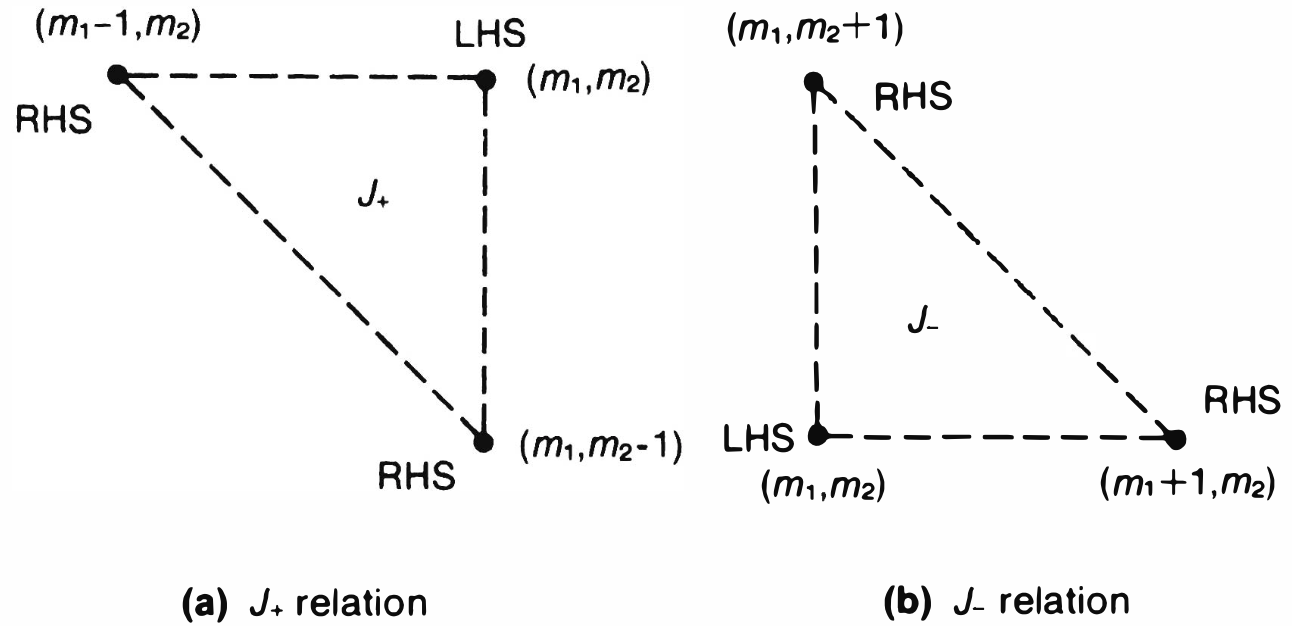
\includegraphics[width=10cm]{AngularMomentum/J+J-relation}
\caption{左图是$J_+$关系,右图是$J_-$关系。分别联系起三个不同的CG因子。}
%\label{default}
\end{center}
\end{figure}

这里$m_1 = -j_1, -j_1 + 1, ..., j_1 -1, j_1$,即在$-j_1$到$j_1$之间间隔为1的分立取值,类似地$m_2$是$-j_2$到$j_2$之间间隔为1的分立取值。如果我们取$m_1$为横轴,$m_2$为纵轴,$(m_1, m_2)$就构成了$m_1  m_2$平面上的一系列格点。每一个格点都代表一个CG系数$\left\langle m_1 ,  m_2 | j, m_1 + m_2 \right\rangle$。

现在我们就可给出角动量$j_1$加角动量$j_2$的所有CG系数的一般步骤。

(1)$j = |j_1 - j_2|, ... j_1 + j_2 -1, j_1 + j_2$;

(2)对某个确定的$j$,$m_1 + m_2  = - j, -j +1, ..., j$;所有非零CG系数被包围在$m_1 = \pm j_1$,$m_2 = \pm j_2$和$m_1 + m_2 = \pm j$这六条直线围成的多边形内。

\begin{figure}[htbp]
\begin{center}
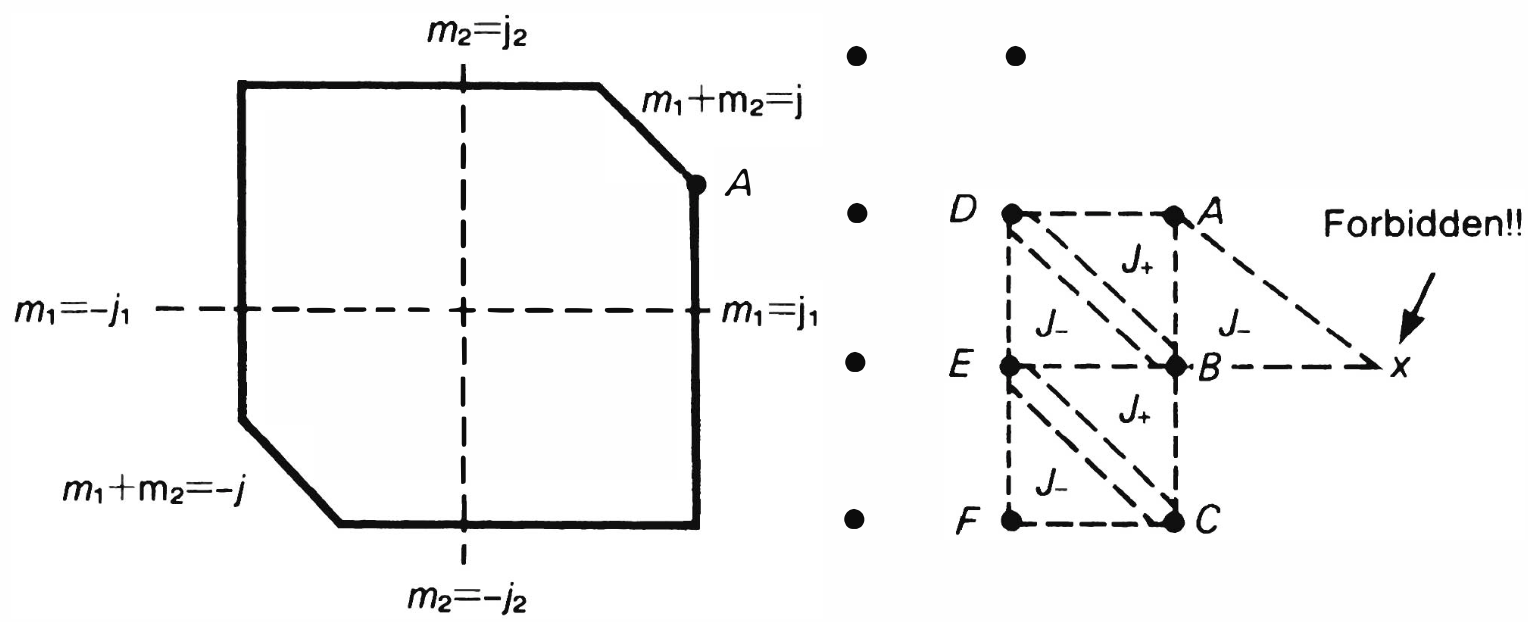
\includegraphics[width=10cm]{AngularMomentum/cgcoeficients.png}
\caption{左图:CG系数不为零的区域;右图:利用$J_{\pm}$关系“递推”CG系数。}
\label{default}
\end{center}
\end{figure}

(3)我们由图中的A点出发,首先构造$J_-$三角形ABX,由于X已经出了CG系数不为零的区域,所以该点的CG系数为0,这样我们就能用A点的CG系数表示B点的CG系数了。然后我们再构造$J_+$三角形ABD,这样D点的CG系数也可以用A点的CG系数来表示了。我们可以一直这么做下去,……直到覆盖整个CG系数不为0的区域,最后再利用归一关系把各点CG系数的取值最终确定下来。


\subsection*{参考}

J. J. Sakurai, Modern Quantum Mechanics, \S 3.5, 3.6, 3.7, 3.8
